\documentclass[a4, oneside]{report}

% twoside twocolumn

%\usepackage[pdftex]{color, graphicx, epsfig}
%\usepackage[final]{pdfpages}

%\usepackage[print]{booklet}

\usepackage{amsmath}
\usepackage[swedish]{babel}
\usepackage{blindtext}
\usepackage{setspace}
\usepackage{graphicx}
\usepackage[utf8]{inputenc}
\usepackage{fancyhdr}
\usepackage{array}
\usepackage[table]{xcolor}
\usepackage{subfiles}
\usepackage{multicol}
\usepackage[bottom]{footmisc}
\usepackage{amsfonts}
\usepackage{pgfplots} 
\usepackage{longdivision}
\usepackage{polynom}
\usepackage[hidelinks]{hyperref}
\usepackage{biblatex}
\usepackage{csquotes}
\usepackage{incgraph,tikz}
\usepackage{tipa}
\pgfplotsset{width=9cm, compat=1.9}
% width=13cm
\addbibresource{../../sources.bib}

\usepackage{listings}



\newcommand{\tikzmark}[1]{\tikz[overlay,remember picture] \node (#1) {};}
\tikzset{square arrow/.style={to path={-- ++(0,-.25) -| (\tikztotarget)}}}


\definecolor{mycolorRED}{RGB}{253,67,53}
\definecolor{mycolorYELLOW}{RGB}{251,188,4}
\definecolor{mycolorGREEN}{RGB}{52,168,83}

\definecolor{codegreen}{rgb}{0,0.6,0}
\definecolor{codegray}{rgb}{0.5,0.5,0.5}
\definecolor{codepurple}{rgb}{0.58,0,0.82}
\definecolor{backcolour}{rgb}{0.96,0.96,0.96}

\definecolor{purple}{rgb}{0.65,0.14,0.64}
\definecolor{lightBlue}{rgb}{0.25,0.47,0.94}
\definecolor{uglyBrown}{rgb}{0,1,0}

\lstdefinestyle{mystyle}{
    backgroundcolor=\color{backcolour},   
    commentstyle=\color{codegreen},
    keywordstyle=\color{magenta},
    keywordstyle=[2]\color{purple},
    keywordstyle=[3]\color{lightBlue},
    keywordstyle=[4]\color{uglyBrown},
    keywordstyle=[5]\color{codegreen},
    keywords=[2]{
        for, int, if, static, public, void, int, bool, while
    },
    keywords=[3]{
        swap, bubbleSort, cocktailSort, Length, multiplyByTwo, combSort, getNextGap
    },
    keywords=[4]{
        1, 2, 3, 4, 5, 6, 7, 8, 9, 0
    },
    keywords=[5]{
        return, break, true, false
    },
    numberstyle=\tiny\color{codegray},
    stringstyle=\color{codepurple},
    basicstyle=\ttfamily\footnotesize,
    breakatwhitespace=false,         
    breaklines=true,                 
    keepspaces=true,                 
    numbers=left,                    
    numbersep=5pt,                  
    tabsize=1,
}
\lstset{style=mystyle}

\begin{document}
\pagenumbering{gobble}

\incgraph[documentpaper][width=\paperwidth]{../../GACover.png}
%width=\paperwidth,height=\paperheight
\newpage

{\color{white} highlighted}
\vfill
{\color{white} highlighted}\\
Erik Viking Norberg 2019\\
erik.norberg@europaskolan.com\\
\textcolor{red}{2020-20-20}

\newpage

\topskip0pt
\vspace*{\fill}
\textcolor{white}{a}\hspace{0.9cm}{\large \textbf{\textit{''Premature optimization is the root of all evil.''}}}\\
\textcolor{white}{a}\hspace{0.9cm}-- D.E. Knuth, The Art of Computer Programming, Volume 1
\vspace*{\fill}

\newpage

\topskip0pt
\vspace*{\fill}
{\large \textbf{\textit{''In some ways, programming is like painting. You start witha blank canvas and certain basic raw materials. You use a combination of science, art, and craft to determine what to do withthem.''}}}\\
-- Andrew Hunt, The Pragmatic Programmer: From Journeyman to Master
\vspace*{\fill}

\newpage

\onecolumn
\pagenumbering{arabic}
\pagestyle{fancy}
\fancyhf{}
\rhead{Erik V. Norberg}
\lhead{Sorteringsalgoritmer}
\cfoot{\thepage}

\pagenumbering{arabic}

\lhead{Abstract}
\section*{Abstract}
\blindtext

\newpage
\lhead{Innehållsförteckning}
\tableofcontents

%\twocolumn
\newpage
\lhead{Introduktion}

\chapter{Inledning}

\section{Introduktion}
Du ska till ett bibliotek och hämta en bok. När du kommer fram till biblioteket börjar du kolla efter den. Men inga av böckerna verkar stå i någon ordning. Då inser du att alla böckerna i biblioteket inte är sorterade. Det är huller om buller. Du frågar då bibliotekarien varför det inte är sorterade. Hon svarar att det tar för lång tid för henne att sortera alla böcker eftersom det har så många, så hon har inte gjort det. Du, med ditt genialiska intellekt, kommer snabbt på att man kan skriva ett dataprogram som sorterar all böckerna snabbare än vad någon människa kan göra. Du utbrister då heureka! Sedan springer du hem och sätter dig framför din dator för att skriva dataprogrammet. Men du inser snabbt att det finns många, många, väldigt många olika sätt att sortera böckerna. Du kommer på ett flertal sätt man kan göra det men du vet inte vilken metod du ska använda. Du ville ju att programmet skulle vara snabbt så du bestämmer dig för att skriva alla metoder du har kommit på för att kunna se vilken som är snabbast. Detta är vad mitt gymnasiearbete kommer att handla om. Vilken metod (eller sorteringsalgoritm som det kallas) är mest effektiv när det kommer till sortering.\\
Inom datavetenskap är en sorteringsalgoritm en algoritm som sorterar element i en lista till en viss ordning. De mest vanliga ordningarna att sortera till är numerisk ordning eller lexikografisk ordning. Effektiv sortering är viktigt för att optimera effektiviteten av andra algoritmer (till exempel sök- och sammanslagningsalgoritmer) som kräver att dess givna data är i sorterad ordning. Sortering är också ofta användbart för kanonisering av data och för att producera mänsklig läsbar data. Mer formellt måste den sorterade datan från en sorteringsalgoritm uppfylla två villkor:\cite{1, 2}
\begin{enumerate}
    \item Den sorterade datan är i icke minskande ordning (varje element är inte mindre än föregående element efter den önskade ordningen);
    \item Resultatet är en permutation (en omordning som behåller alla original element) av den givna datan.
\end{enumerate}
Vidare lagras ingångsdata ofta i en matris, vilket tillåter slumpmässig åtkomst av dess element, snarare än en lista, som endast tillåter sekventiell åtkomst; även om många algoritmer kan tillämpas på vilken typ av data som helst efter lämplig modifiering.\\
Redan från början av datavetenskapen har sortering attraherat mycket forskning, kanske på grund av att det är ett problem som är lätt att konceptuellt förstå men är väldigt svårt att lösa. Blandet det första personerna som skrev sorteringsalgoritmer är Betty Holberton som skrev ENIAC och UNIVAC. En av det mest kända sorteringsalgoritmerna \textit{“Bubble sort”} skrevs redan så tidigt som 1956. Detta innebär att ämnet redan är väldigt väl undersökt. Så jag kommer inte kunna skriva någon ny sorteringsalgoritm men jag kommer kunna analysera det som redan finns. \cite{1} Mer exakt kommer jag analysera: \textit{Selection sort, Shellsort, Insertion Sort, Merge Sort, Quick Sort, Heap Sort, Bubble Sort, Comb sort} och \textit{Bidirectional Bubble Sort}.

\section{Syfte och metod}
Syftet med arbetet är att bestämma den snabbaste och mest effektiva sorteringsalgoritmen. Detta kommer redovisat genom att först visa hur man kan skriva algoritmerna i programmeringsspråket C\#. Det är viktigt att man förstår hur syntaxen i C\# fungerar så det kommer läggas fokus på hur den fungerar och vad den gör. Om man inte förstår koden är det svårt för en att förstå resten av arbetet eftersom C\# är grunden för arbetet. Följt av detta kommer matematiken bakom algoritmernas ordo (se sida 5) förklaras så att man från ett matematiskt perspektiv kan jämföra algoritmerna.\\
Sorteringsalgoritmer i sin helhet öppnar upp många intressanta dörrar inom datavetenskapen. Men det är ett träsk av information och data som är omöjlig att utforska på en och samma gång. För att undvika det träsket kommer jag begränsa arbetet till enbart så kallade \textit{“Comparison sorting algorithms”} och inte \textit{“Non-Comparison sorting algorithms”} (eller andra former av sorteringsalgoritmer).\\
Sorteringsalgoritmer handlar inte bara om optimering utan också och om minneshantering inom RAM minnet. Särskilt dom sorteringsalgoritmer som är \textit{"på plats"}. Det innebär att det bara behöver $\mathcal{O}(1)$ eller $\mathcal{O}(\log{n})$ minne (beteckningen $\mathcal{O}$ förklaras mer på sida 5) utöver det element som sorteras och det behöver inte skapa temporära platser att spara datan i RAM minnet som andra algoritmer behöver göra. \cite{3} Dock så är frågan om minne inte viktigt för arbetet så jag kommer undvika frågan om minne.

\section{Bakgrund}
\lhead{Bakgrund}
För att man ska kunna analysera algoritmerna måste man först förstå ett par fundamentala saker. Ordo, så att man kan jämföra dom matematiskt, C\# syntax, så man förstår implementationerna av algoritmerna, och visa termer som kommer uppstå ett flertal gånger i arbetet.
\subsection{Ordo}%['ɔr doʊ]
Ordo (\textit{Ordning} på latin. Utalat \textipa{'\textopeno r do\textscomega}) är ett begrepp inom matematiken och även datavetenskapen som används för att ge ett mått på hur beräkningsmässigt tung en funktion är. Detta betecknas med ett versalt $\mathcal{O}$. När en funktion beskrivs med ordo så beskrivs vanligtvist en övre gräns för en funktions tillväxthastighet. Det vill säga hur snabbt $y$ ökar med ett ökande $x$. Till exempel betecknar $\mathcal{O}(x^2)$ och $\mathcal{O}(\sqrt{x})$ något som växer lika fort som $x^2$ respektive $\sqrt{x}$ då $x$ ökar. Detta används särskilt inom datavetenskapen när man beskriver hastigheten av olika algoritmer, som sorteringsalgoritmer. \cite{4, 5} Associerat med $\mathcal{O}$ är ett par andra notationer som använder symbolerna $o$, $\Omega$, $\omega$ och $\Theta$ som beskriver andra gränser av asymptotisk tillväxt. Dessa kommer vi gå igenom mer i detalj snart.\\
En mer formell definitionen av ordo lyder: Låt $f$ vara en reell eller komplex funktion och $g$ vara en reell funktion. Låt båda funktionerna vara definierade med någon begränsad delmängd av det positiva reella talen och $g(x)$ vara strikt positivt för stora $x$. Man skriver \cite{6}
\begin{equation*}
    f(x)=\mathcal{O}(g(x))\hspace{5mm}\text{när }x\rightarrow\infty
\end{equation*}
om absolutbeloppet av $f(x)$ är en positiv konstant multiple av $g(x)$ för alla stora värden av $x$. Alltså är $f(x)=\mathcal{O}(g(x))$ om det existerar ett positivt reellt number $M$ och reellt numer $x_0$ så att
\begin{equation*}
    |f(x)|\leq Mg(x)\hspace{5mm}\text{för alla }x\leq x_0.
\end{equation*}
I många sammanhang lämnas antagandet att vi är intresserade av tillväxthastigheten när variabeln x går mot oändlighet, då skriver man mer enkelt
\begin{equation*}
   f(x)=\mathcal{O}(g(x)).
\end{equation*}
Ordo kan även användas för att beskriva betendet av $f$ nära ett reelt number $a$ (ofta $a=0$). Man skriver
\begin{equation*}
   f(x)=\mathcal{O}(g(x))\hspace{5mm}\text{när }x\rightarrow a
\end{equation*}
om det existerar ett positivt nummer $\delta$  och $M$ sådan att för alla $x$ med $0<|x-a|<\delta$ så är
\begin{equation*}
   |f(x)|\leq Mg(x).
\end{equation*}
Eftersom $g(x)$ är valt att vara noll för värden på $x$ tillräckligt nära $a$, kan båda dessa definitioner förenas med användning av \textit{limit superior}:
\begin{equation*}
   f(x)=\mathcal{O}(g(x))\hspace{5mm}\text{när }x\rightarrow a
\end{equation*}
om
\begin{equation*}
   \limsup_{x\rightarrow a}\frac{|f(x)|}{g(x)}<\infty.
\end{equation*}
Det tidigare nämnda notationerna $o$, $\Omega$, $\omega$ och $\Theta$ kan man lätt förstå i tabellen under då det inte krävs några formella bevis för att förklara dem, eftersom det är så lika $\mathcal{O}$. 
\begin{table}[h!]
    \centering
    \begin{tabular}{|l|l|}
    \hline
    \rowcolor[HTML]{A4C2F4} 
    \multicolumn{1}{|c|}{\cellcolor[HTML]{A4C2F4}{\color[HTML]{000000} Notation}} & \multicolumn{1}{c|}{\cellcolor[HTML]{A4C2F4}{\color[HTML]{000000} I ord}} \\ \hline
    \rowcolor[HTML]{FFFFFF} 
    $f(n)\in\mathcal{O}(g(n))$                                                    & $f$ växer högst lika snabbt som $g$                                       \\ \hline
    \rowcolor[HTML]{F3F3F3} 
    $f(n)\in\Omega(g(n))$                                                         & $f$ växer minst lika snabbt som $g$                                       \\ \hline
    \rowcolor[HTML]{FFFFFF} 
    $f(n)\in\Theta(g(n))$                                                         & $f$ växer lika snabbt som $g$                                             \\ \hline
    \rowcolor[HTML]{F3F3F3} 
    $f(n)\in o(g(n))$                                                             & $f$ växer långsammare än $g$                                              \\ \hline
    \rowcolor[HTML]{FFFFFF} 
    $f(n)\in\omega(g(n))$                                                         & $f$ växer snabbare än $g$                                                 \\ \hline
    \end{tabular}
    \caption{Ordo och relaterade notationer}
\end{table}\\

Som nämnt innan beskriver ordo hur beräkningsmässigt  tung  en  funktionär. Detta är väldigt viktigt när det kommer till analys och optimering av olika algoritmer, främst när det ska jämföras med varandra. Om vi har funktionen $f(x)=6x^4-2x^3+5$ och vi vill förenkla den med ordo så vi kan se hur den växer när $x$ går mot oändligheten så börjar vi med att kolla på termerna av $f$, nämligen $6x^4$, $-2x^3$ och $5$. Utav dessa tre termer har termen med den största exponenten med avseende på $x$ snabbast tillväxthastighet, nämligen $6x^4$. $6x^4$ är en produkt av $6$ och $x^4$ där första termen inte är beroende av $x$. Att utelämna denna term resulterar i en förenklad formen $x^4$. Således säger vi att $f(x)=\mathcal{O}(x^4)$.\\
Det finns några par tillväxthastigheter som man stöter på oftast när man talar om ordo. Det är dessa följande:
\begin{center}
  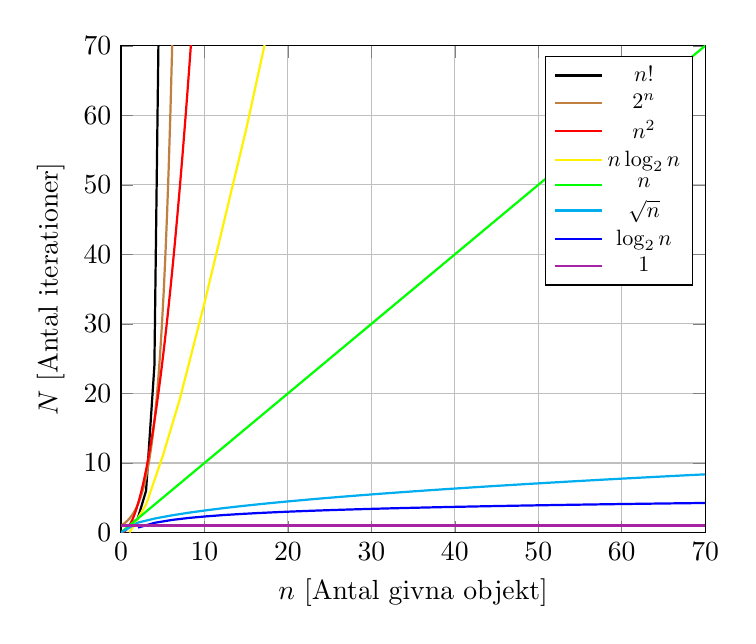
\begin{tikzpicture}
      \begin{axis}[
      xlabel = {$n$ [Antal givna objekt]},
      ylabel = {$N$ [Antal iterationer]},
      %
      xmin = 0, 
      xmax = 70,
      ymin = 0, 
      ymax = 70,
      %
      xmajorgrids = true,
      ymajorgrids = true,
      %
      legend style={nodes={scale=0.8, transform shape}}
      ]
      \addplot [color=black,  thick] coordinates { (0,1) (1,1) (2,2) (3,6) (4, 24) (5,120) };
      \addplot [domain=0:10,  samples=50, color=brown, thick]{2^x};
      \addplot [domain=0:10,  samples=50, color=red, thick]{x^2};
      \addplot [color=yellow, thick] coordinates { (1,0) (3,4) (5,11) (7,19) (10,33) (12,43) (15,58) (17,69) (20,86) (22,98) (25,116) (30,147)};
      \addplot [domain=0:100, samples=50, color=green, thick]{x};
      \addplot [domain=0:100, samples=50, color=cyan, thick]{sqrt(x)};
      \addplot [domain=0:100, samples=50, color=blue, thick]{ln(x)};
      \addplot [color=purple, thick] coordinates { (0,1) (100,1)};
      %
      \addlegendentry{$n!$}
      \addlegendentry{$2^n$}
      \addlegendentry{$n^2$}
      \addlegendentry{$n\log_2n$}
      \addlegendentry{$n$}
      \addlegendentry{$\sqrt{n}$}
      \addlegendentry{$\log_2n$}
      \addlegendentry{$1$}
      \end{axis}
  \end{tikzpicture}
\end{center}

\subsection{Fundamental C\#}
C\# (C-Sharp) är ett programmeringsspråk utvecklat av Microsoft som körs på .NET Framework \cite{7}. C\# är i första hand ett objektorienterat programspråk. Även kallad ett OOP (från engelskans \textit{Object Oriented Programming}). Det är varför detta arbete skrivs i C\#. Då alla sorteringsalgoritmer kan skrivas som var sitt objekt. Ett objekt är en instans av samlad syntax som används för att utföra en given operation. Exempelvis kan ett objekt kallas på för att göra en viss beräkning eller för att sammanställa data. En objekt i C\# kan se ut såhär:
\begin{lstlisting}[style=mystyle, numbers=left]
 public void multiplyByTwo(int n)
 {
   return n * 2;
 }
\end{lstlisting}
Denna funktion tar in ett heltal, \lstinline{int n}, och ger tillbaka ett heltal dubbelt så stort som \lstinline{n}, \lstinline{return n * 2}.\\
En funktion i C\# måste inte bara behandla aritmetik. En funktion kan även behandla arrays (listor) vilket är väldigt användbart när man vill sortera. Exempelvis om vi har listan
\begin{lstlisting}[style=mystyle, numbers=none]
 int[] lista = {1, 2, 5, 3, 4};
\end{lstlisting}
och vi vill byta plats på fyran och femman för att få listan i storleksordning kan vi skriva en funktion som denna:
\begin{lstlisting}[style=mystyle, numbers=left]
 static void swap(int x, int y, int[] arr)
 {
   int temp = arr[x];
   arr[x] = arr[y];
   arr[y] = temp;
 }
\end{lstlisting}
Den tar in två positioner \lstinline{x} och \lstinline{y} i en given lista \lstinline{arr} och byter plats på dom. Den göra detta genom att spara heltalet på position \lstinline{x} i \lstinline{arr} inuti en temporär variabel \lstinline{temp}. När \lstinline{x} är sparad i \lstinline{temp} överskrider funktionen \lstinline{x} med \lstinline{y}. Sist överskrider funktionen \lstinline{y} med \lstinline{temp}. Då har det två positionerna byt plats. Vi kallar på funktionen för att byta plats på fyran och trean i \lstinline{lista}:
\begin{lstlisting}[style=mystyle, numbers=none]
 swap(3, 5, lista);
\end{lstlisting}
och vi får att listan nu är 
\begin{lstlisting}[style=mystyle, numbers=none]
 [1, 2, 3, 4, 5]
\end{lstlisting}
Observera att \lstinline{swap} inte har en \lstinline{return}, såsom \lstinline{multiplyByTwo} har på rad $3$. Detta är då för att \lstinline{swap} inte ger tillbaka en ny lista. Den ändrar den givna arrayn utan att skapa en ny array medans \lstinline{multiplyByTwo} tar in ett heltal och ger tillbaka ett nytt heltal. Observera även att när vi kallar på \lstinline{swap} ger vi den $3$ och $4$ då det är positionerna av numrena vi vill byta plats på, inte för att det är $3$ och $4$ vi vill byta plats på. Om vi istället ville byta plats på $1$ och $3$ hade vi skrivit
\begin{lstlisting}[style=mystyle, numbers=none]
 swap(1, 4, lista);
\end{lstlisting}
Vilket hade gett
\begin{lstlisting}[style=mystyle, numbers=none]
 [3, 2, 4, 1, 5]
\end{lstlisting}
Funktion \lstinline{swap} kommer användas för varje sorteringsalgoritm som arbetet kommer analysera. Alltså varje gång en sorteringsalgoritm kallar på \lstinline{swap} kommer den kalla koden som är beskriven ovan.

\subsection{Grundläggande algoritmer}
Sorteringsalgoritmer kan vara väldigt komplexa och effektiva med bekosnad av att vara väldigt svåra att förstå. Docks så kan sorteringsalgoritmer vara väldigt simpla men med bekostnad av att vara mindre effektiva. Ett par simpla sorteringsalgoritmer vi kommer kolla på nu är \textit{Bubblesort}, \textit{Cocktailsort} och, \textit{Shellsort}. Vi börjar med Bubblesort.\\
Bubblesort är bland det minst effektiva sorteringsalgoritmerna men den är ändå en av det mest kända sorteringsalgoritmerna eftersom den är sorteringsalgoritmernas \textit{“Hello World”}. Den är väldigt lätt att förstå både praktiskt och teoretiskt. Därför används den mest som ett pedagogiskt verktyg \cite{8}. Bubblesort fungerar genom att jämföra intilliggande element i en lista. Om elementen som jämförs ligger i fel ordning byter det plats så att det större elementet rör sig uppåt i listan. Denna process fortsätter tills det största elementet i listan är högst upp i listan. När detta är klart börjar algoritmen om men för det näst största elementet i listan. Detta repeteras till listan är sorterad. Låt oss säga att vi har en array 
\begin{lstlisting}[style=mystyle, numbers=none]
 int[] lista = {5, 1, 4, 2, 8};
\end{lstlisting}
som ska sorteras från minst till störst med Bubblesort. Det kommer bara ta tre iterationer för bubblesort att sortera arrayen (elementen skrivna i fetstil jämförs);\\\\
\textbf{Första iterationen:}
\begin{align*}
    [\textbf{5}, \textbf{1}, 4, 2, 8] &\rightarrow [\textbf{1}, \textbf{5}, 4, 2, 8]\\
    [1, \textbf{5}, \textbf{4}, 2, 8] &\rightarrow [1, \textbf{4}, \textbf{5}, 2, 8]\\
    [1, 4, \textbf{5}, \textbf{2}, 8] &\rightarrow [1, 4, \textbf{2}, \textbf{5}, 8]\\
    [1, 4, 2, \textbf{5}, \textbf{8}] &\rightarrow [1, 4, 2, \textbf{5}, \textbf{8}]
\end{align*}
\textbf{Andra iterationen:}
\begin{align*}
    [\textbf{1}, \textbf{4}, 2, 5, 8] &\rightarrow [\textbf{1}, \textbf{4}, 2, 5, 8]\\
    [1, \textbf{4}, \textbf{2}, 5, 8] &\rightarrow [1, \textbf{2}, \textbf{4}, 5, 8]\\
    [1, 2, \textbf{4}, \textbf{5}, 8] &\rightarrow [1, 2, \textbf{4}, \textbf{5}, 8]
\end{align*}
Vid detta laget är arrayen redan sorterad men det vet inte algoritmen. Den måste iterera över arrayen utan att behöva byta några element för att veta att den är klar.\\\\
\textbf{Tredje iterationen:}
\begin{align*}
    [\textbf{1}, \textbf{2}, 4, 5, 8] &\rightarrow [\textbf{1}, \textbf{2}, 4, 5, 8]\\
    [1, \textbf{2}, \textbf{4}, 5, 8] &\rightarrow [1, \textbf{2}, \textbf{4}, 5, 8]
\end{align*}
Denna algoritm är lätt att implementera i C\# då den inte kräver mycket kod för att utföras:
\begin{lstlisting}[style=mystyle, numbers=left]
 static void bubbleSort(int[] array)
 {
   items = array.Length;
   for (int i = 0; i < items; i++)
   {
     for (int j = 0; j < items - i - 1; j++)
     {
       if (array[j] > array[i])
       {
         swap(i, j, array);
       }
     }
   }
 }
\end{lstlisting}
Vi initialiserar funktionen på rad $1$. Vi kallar funktionen för \lstinline{bubbleSort} och säger även att den bara kan ta emot en endimensionell array. Väl inuti funktionen säger vi att \lstinline{items} ska vara lika med hur många element som finns i \lstinline{array} när den är given. Detta är inte nödvändigt men det gör koden mer läsbar. Nu vill vi kunna iterera över \lstinline{array} lika många gånger som det finns element i \lstinline{array} men för varje iteration vill vi iterera över ett element mindre. Detta gör vi med \lstinline{for} looparna på rad $4$ och $6$. Första \lstinline{for} loopen på rad $4$ loopar över alla element i \lstinline{array} och på samma gång ökar värdet av \lstinline{i} tills den är lika stor som \lstinline{items}. Inuti den \lstinline{for} loopen är en nested\footnote{Det är en loop innuti en annan loop. Nästlade loop'ar är inte direkt ovanliga speciellt vid algoritmer som behandlar data. Exempel kan vara vid uppritning av kartor i grafiska spel eller sortering av data.} \lstinline{for} loop på rad $6$ som också itererar över alla element i \lstinline{array} förutom det \lstinline{i} sista elementen. Med detta kan vi jämföra elementen på plats \lstinline{i} och \lstinline{j} för att se vilken som är störst. Om \lstinline{j} är större än \lstinline{i} bytter det plats, detta gör vi på rad $8$ till $11$.\\
Nu kan vi kalla på \lstinline{bubbleSort} för att sortera \lstinline{lista}:
\begin{lstlisting}[style=mystyle, numbers=none]
 bubbleSort(lista);
\end{lstlisting}
Vilket sorterar \lstinline{lista} så att den nu är:
\begin{lstlisting}[style=mystyle, numbers=none]
 [1, 2, 4, 5, 8]
\end{lstlisting} 
Analysen av  Bubblesort är inte särskilt svår heller. Om vi har en array som är $n$ element lång så kommer Bubblesort behöva jämföra $(n-1)$ element första iteration. Andra iterationen kommer den behöva jämföra $(n-2)$ element. Tredje Iterationen kommer den behöva jämföra $(n-3)$ element och så vidare. Detta innebär att den totala mängden jämförelser  bubblesort kommer behöva göra är
\begin{equation*}
    (n-1) + (n-2) + \cdots + 2 + 1 = \sum\frac{n(n-1)}{2}
\end{equation*}
Vilket betyder att bubblesort har ett ordo av $\mathcal{O}(n^2)$.\\

Som sagt är Bubblesort inte särskilt effektiv. Man kan optimera koden så att den blir lite mer effektiv men det gör ingen jättestor skillnad. Man kan dock förbättra själva algoritmen. Första sättet man kanske kommer på för att förbättra algoritmen är genom att ändra hur den itererar genom en array. Istället för att varje iteration ska genomföras från vänster till höger en gång i en array innan nästa iteration kan varje iteration genomföras från vänster till höger och sedan tillbaka. Detta minskar hur många iterationer som krävs för att sortera en array eftersom den inte bara flyttar det största elementen till toppen av listan, den flyttar även samtidigt den minsta elementet till botten av listan per iteration. Denna typ av sorteringsalgoritm kallas för \textit{Bidirectional Bubblesort} eller \textit{Cocktailsort} som den är mer känd som. Låt oss säga att vi har samma array som för Bubblesort
\begin{lstlisting}[style=mystyle, numbers=none]
 int[] lista = {5, 1, 4, 2, 8};
\end{lstlisting}
som ska sorteras med Cocktailsort. Det kommer bara ta två iterationer för Cocktailsort att sortera arrayen (elementen  skrivna  i  fetstil jämförs);\\\\
\textbf{Första iterationen:}
\begin{align*}
    [\textbf{5}, \textbf{1}, 4, 2, 8] &\rightarrow [\textbf{1}, \textbf{5}, 4, 2, 8]\\
    [1, \textbf{5}, \textbf{4}, 2, 8] &\rightarrow [1, \textbf{4}, \textbf{5}, 2, 8]\\
    [1, 4, \textbf{5}, \textbf{2}, 8] &\rightarrow [1, 4, \textbf{2}, \textbf{5}, 8]\\
    [1, 4, 2, \textbf{5}, \textbf{8}] &\rightarrow [1, 4, 2, \textbf{5}, \textbf{8}]\\
    [1, 4, \textbf{2}, \textbf{5}, 8] &\rightarrow [1, 4, \textbf{2}, \textbf{5}, 8]\\
    [1, \textbf{4}, \textbf{2}, 5, 8] &\rightarrow [1, \textbf{2}, \textbf{4}, 5, 8]\\
    [\textbf{1}, \textbf{2}, 4, 5, 8] &\rightarrow [\textbf{1}, \textbf{2}, 4, 5, 8]
\end{align*}
Vid  detta  laget är  arrayen  redan  sorterad  men  det  vet  inte  algoritmen.  Den måste iterera över arrayen utan att behöva byta några element för att veta att den är klar.\\\\
\textbf{Andra iterationen:}
\begin{align*}
    [1, \textbf{2}, \textbf{4}, 5, 8] &\rightarrow [1, \textbf{2}, \textbf{4}, 5, 8]\\
    [1, 2, \textbf{4}, \textbf{5}, 8] &\rightarrow [1, 2, \textbf{4}, \textbf{5}, 8]\\
    [1, \textbf{2}, \textbf{4}, 5, 8] &\rightarrow [1, \textbf{2}, \textbf{4}, 5, 8]
\end{align*}
Denna algoritm är inte mycket svårare att implementera i C\# än vad Bubblesort är:
\begin{lstlisting}[style=mystyle, numbers=left]
 static void cocktailSort(int[] array)
 {
   int start = 0;
   int end = array.Length;
   bool swapped = true;
   
   while (swapped) 
   {
     for (int i = start; i < end - 1; i++)
     {
       if (array[i] > array[i + 1])
       {
         swap(i, i + 1, array);
         swapped = true;
       }
     }
     if (swapped == false)
     {
       break;
     }
     swapped = false;
     end -= 1;
     for (int i = end - 1; i >= start; i--)
     {
       if (array[i] > array[i + 1])
       {
         swap(i, i + 1, array);
         swapped = true;
       }
     }
     start += 1;
   }
 }
\end{lstlisting}
Vi initialiserar funktionen på rad $1$. Vi kallar funktionen för \lstinline{cocktailSort} och säger även att den bara kan ta emot en endimensionell array. Väl inuti funktionen säger vi att \lstinline{start} och \lstinline{end} ska vara $0$ respektive längden av \lstinline{arr}. Dessa variabler kommer avgöra vart initierandet kommer börja och sluta. Vi skapar även en boolean \lstinline{swapped} som kommer avgöra om \lstinline{arr} är sorterad. På rad $7$ börjar en \lstinline{while} loop som kommer loopa tills \lstinline{swapped} är falsk. Det första som händer i \lstinline{while} loopen är att \lstinline{for} loopen på rad $9$ itererar över \lstinline{arr} från vänster (med start på \lstinline{start} positionen) till höger (med slut vid \lstinline{end} positionen) och jämför elementet den är på med elementet till höger och byter dom ifall det behövs. Den sätter även \lstinline{swapped} som san ifall den behövde byta plats på två element. Följt av den \lstinline{for} loopen är det ett \lstinline{if} statement på rad $17$ som stannar \lstinline{while loopen} om \lstinline{swapped} är falsk. Det vill säga listan är sorterad. Men om den inte är sorterad kommer nästa \lstinline{for} loop på rad  $23$ att börja. Den fungerar samma som \lstinline{for} loopen på rad $9$ förutom att det itererar över \lstinline{arr} från vänster till höger istället. Observera att den loopen kommer ignorera objektet längsta till höger i \lstinline{arr} på grund av \lstinline{start} och \lstinline{end} på rad $22$ och $31$.\\
Nu kan vi kalla på \lstinline{cocktailSort} för att sortera \lstinline{lista}:
\begin{lstlisting}[style=mystyle, numbers=none]
 cocktailSort(lista);
\end{lstlisting}
Vilket sorterar \lstinline{lista} så att den nu är:
\begin{lstlisting}[style=mystyle, numbers=none]
 [1, 2, 4, 5, 8]
\end{lstlisting}
Tidskomplexiteten av Cocktailsort är samma som för Bubblesort. En iteration av Cocktailsort är samma som två iterationer av Bubblesort. Om vi har en array som är $n$ element lång så kommer första iterationen av Cocktailsort behöver jämföra först $(n-1)$ element och sedan $(n-2)$ element (detta är ju då på grund av det två \lstinline{for} looparna på raderna $9$ och $23$). Andra iterationen kommer Coctailsort behöva jämföra  $(n-3)$ sedan $(n-4)$ och så vidare. Detta betyder att den totala summan av iterationer för $n$ element är 
\begin{equation*}
  (n-1) + (n-2) + \cdots + 2 + 1 = \sum\frac{n(n-1)}{2}.
\end{equation*}
Vilket betyder att Coctailsort har ett ordo av $\mathcal{O}(n^2)$.\\

Både Bubblesorts och Coctailsorts hastighet lider främst på grund av att små värden i början eller slutet i deras respektive listor eftersom det tar längst tid att flytta till rätt plats. Såna värden kallas ibland för \textit{turtles}. Stora värden nära början eller slutet av en lista kan även kallas för \textit{rabbits} eftersom det går snabbast att flytta till rätt plats. Combsorts (vilket är den sista grundläggande algoritmen vi kommer kolla på) syfte är att eliminera rabbits och turtles \cite{10}. När två element jämförs med bubblesort har de alltid ett mellanrum (avstånd från varandra) av ett. Ideen med combsort är att mellanrummet kan vara mer än ett. Den inre loopen av bubblesort som byter plats på elementen är modifierad sådan att mellanrummet mellan den jämförda elementen är minskad med en \textit{krympnings faktor} $k$ \cite{9}.  Låt oss säga att vi har en array
\begin{lstlisting}[style=mystyle, numbers=none]
 int[] lista = {5, 1, 4, 2, 8};
\end{lstlisting}
som ska sorteras med Coctailsort. Mellanrummet mellan det jämförda elementen är lika med hur många element som finns i listan. Vi säger även att $k=1$. Det vill säga att mellanrummet kommer bli ett mindre per iteration. Det betyder att den första iterationen kommer se ut såhär (elementen skrivna i fetstil jämförs):\\\\
\textbf{Första iterationen:}
\begin{align*}
    [\textbf{5}, 1, 4, 2, \textbf{8}] &\rightarrow [\textbf{5}, 1, 4, 2, \textbf{8}]
\end{align*}
Det yttersta elementen jämförs eftersom mellanrummet börjar med att vara lika stort som lista är lång.\\\\
\textbf{Andra iterationen:}
\begin{align*}
    [\textbf{5}, 1, 4, \textbf{2}, 8] &\rightarrow [\textbf{2}, 1, 4, \textbf{5}, 8]\\
    [2, \textbf{1}, 4, 5, \textbf{8}] &\rightarrow [2, \textbf{1}, 4, 5, \textbf{8}]
\end{align*}
Här är mellanrummet ett mindre eftersom vi valde att $k$ skulle vara ett. Observera att $k$ vanligtvis inte är ett. $k$ brukar vanligast vara lika med $1.3$. Detta går vi mer in på detalj snart.\\\\
\textbf{Tredje iterationen:}
\begin{align*}
    [\textbf{2}, 1, \textbf{4}, 5, 8] &\rightarrow [\textbf{2}, 1, \textbf{4}, 5, 8]\\
    [2, \textbf{1}, 4, \textbf{5}, 8] &\rightarrow [2, \textbf{1}, 4, \textbf{5}, 8]\\
    [2, 1, \textbf{4}, 5, \textbf{8}] &\rightarrow [2, 1, \textbf{4}, 5, \textbf{8}]
\end{align*}
\textbf{Fjärde iterationen:}
\begin{align*}
    [\textbf{2}, \textbf{1}, 4, 5, 8] &\rightarrow [\textbf{1}, \textbf{2}, 4, 5, 8]\\
    [1, \textbf{2}, \textbf{4}, 5, 8] &\rightarrow [1, \textbf{2}, \textbf{4}, 5, 8]\\
    [1, 2, \textbf{4}, \textbf{5}, 8] &\rightarrow [1, 2, \textbf{4}, \textbf{5}, 8]\\
    [1, 2, 4, \textbf{5}, \textbf{8}] &\rightarrow [1, 2, 4, \textbf{5}, \textbf{8}]
\end{align*}
Denna sista iteration iteration är exakt samma som bubblesort då $k$ har minskat mellanrummet till bara ett.\\
Innan vi kan börja skriva combsort måste vi skriva en funktion som kan krympa mellanrummet mellan det elementen som jämförs. Vi börjar med att initialisera $k$ som en variabel
\begin{lstlisting}[style=mystyle, numbers=none]
 int k = array.Length
\end{lstlisting}
Vi initialiserar den lika lång som \lstinline{items}. Nu kan vi skriva en funktion som krymper mellanrummet med $k$:
\begin{lstlisting}[style=mystyle, numbers=left]
 static int getNextGap(int gap)
 {
   gap = (gap * 10) / 13;
   if (k < 1)
   {
     return 1;
   {
   return gap;
 }
\end{lstlisting}
Denna funktion kommer krympa mellanrummet med $1.3$. Det kan verka slumpmässigt att $k$ ska vara $1.3$ men det har visat sig att $1.3$ är det värde som ger optimalt hastighet för att sortera en array oavsett arrayens storlek. Vi kan nu skriva combsort.
\begin{lstlisting}[style=mystyle, numbers=left]
 static void combSort(int[] array)
 {
  bool swapped = true;
  
   while (gap != 1 || swapped == true)
   {
     gap = getNextGap(gap);
     swapped = false;

     for (int i = 0; i < items - gap; i++)
     {
       if (list[i] > list[i + gap ])
       {
         swap(i, i + gap, list);
         swapped = true;
       }
     }
   }
 }
\end{lstlisting}
Först på rad $3$ har vi en \lstinline{bool} kallad \lstinline{swapped}. Den används för att avgöra om listan är sorterad eller inte då på rad $5$ används den som ett argument för \lstinline{while} loopen. \lstinline{while} loopen kommer att loopa så länge $\text{\lstinline{gap}}\neq1$ och \lstinline{swapped} är san. Det innebär att \lstinline{while} loopen kommer sluta när arrayen är sorterad. Först i \lstinline{while} loopen bestäms mellanrummet mellan det jämförda variablerna med \lstinline{getNextGap} funktionen. Varje loop i \lstinline{while} loopen kommer mellanrummet krympa med $1.3$. Sen kommer en \lstinline{for} loop gör självaste sorteringen. Observera hur lik \lstinline{bubbleSort} den är. Det enda som skiljer dom åt är $k$ och  \lstinline{swapped}.\\
Vi kan nu kalla på \lstinline{combSort} för att sortera \lstinline{lista}:
\begin{lstlisting}[style=mystyle, numbers=none]
 combSort(lista);
\end{lstlisting}
Vilket sorterar listan så att den nu är:
\begin{lstlisting}[style=mystyle, numbers=none]
 [1, 2, 4, 5, 8]
\end{lstlisting}
Tidskomplexiteten av Combsort är rätt så knepig att bevisa.Dock har Paul Vitanyi bevisat med Kolmogorov complexity att den har en tidskomplexitet av $\mathcal{O}(n^2)$ på sida 16 i hans artikel \textit{“Analysis of Sorting Algorithms by Kolmogorov Complexity”} \cite{11}.
 
\subsection{Divide-and-conquer algoritmer (\#2)}
Det algoritmerna vi har kollat på hittills har alla varit väldigt simpla och ineffektiv, vilket vi har sett då alla har haft $\mathcal{O}(n^2)$. Så nu ska vi kolla på Quicksort och Mergesort. Båda är betydligt mycket mer komplexa algoritmer men det är båda väldigt eleganta lösningar till sortering. Båda algoritmerna är så kallade \textit{“Divide-and-conquer”} algoritmer (förkortat DAC). I datavetenskap är DAC ett algoritmiskt paradigm. En DAC algoritm rekursivt delar upp ett problem till två eller flera delproblem av samma eller relaterad typ, tills delproblemen går att lösa omedelbart utan flera delningar. Lösningarna av alla delproblem kombineras sedan för att ge lösning på det ursprungliga problemet \cite{12}.
Eftersom DAC löser delproblem rekursivt måste varje delproblem vara mindre än orginal problemet, och det måste finnas ett grundläggande fall för delproblem. Man kan tänka sig att DAC algoritmer har tre steg:
\begin{enumerate}
   \item \textbf{Dela} upp problemet i ett antal delproblem som är mindre fall av samma problem.
   \item \textbf{Erövra} delproblemen genom att lösa dem rekursivt.
   \item \textbf{Kombinera} det lösta delproblemen tills man löst original problemet.
\end{enumerate}
Om en DAC algoritm skulle lösa ett problem med en rekursioner skulle det se ut såhär:
\begin{center}
  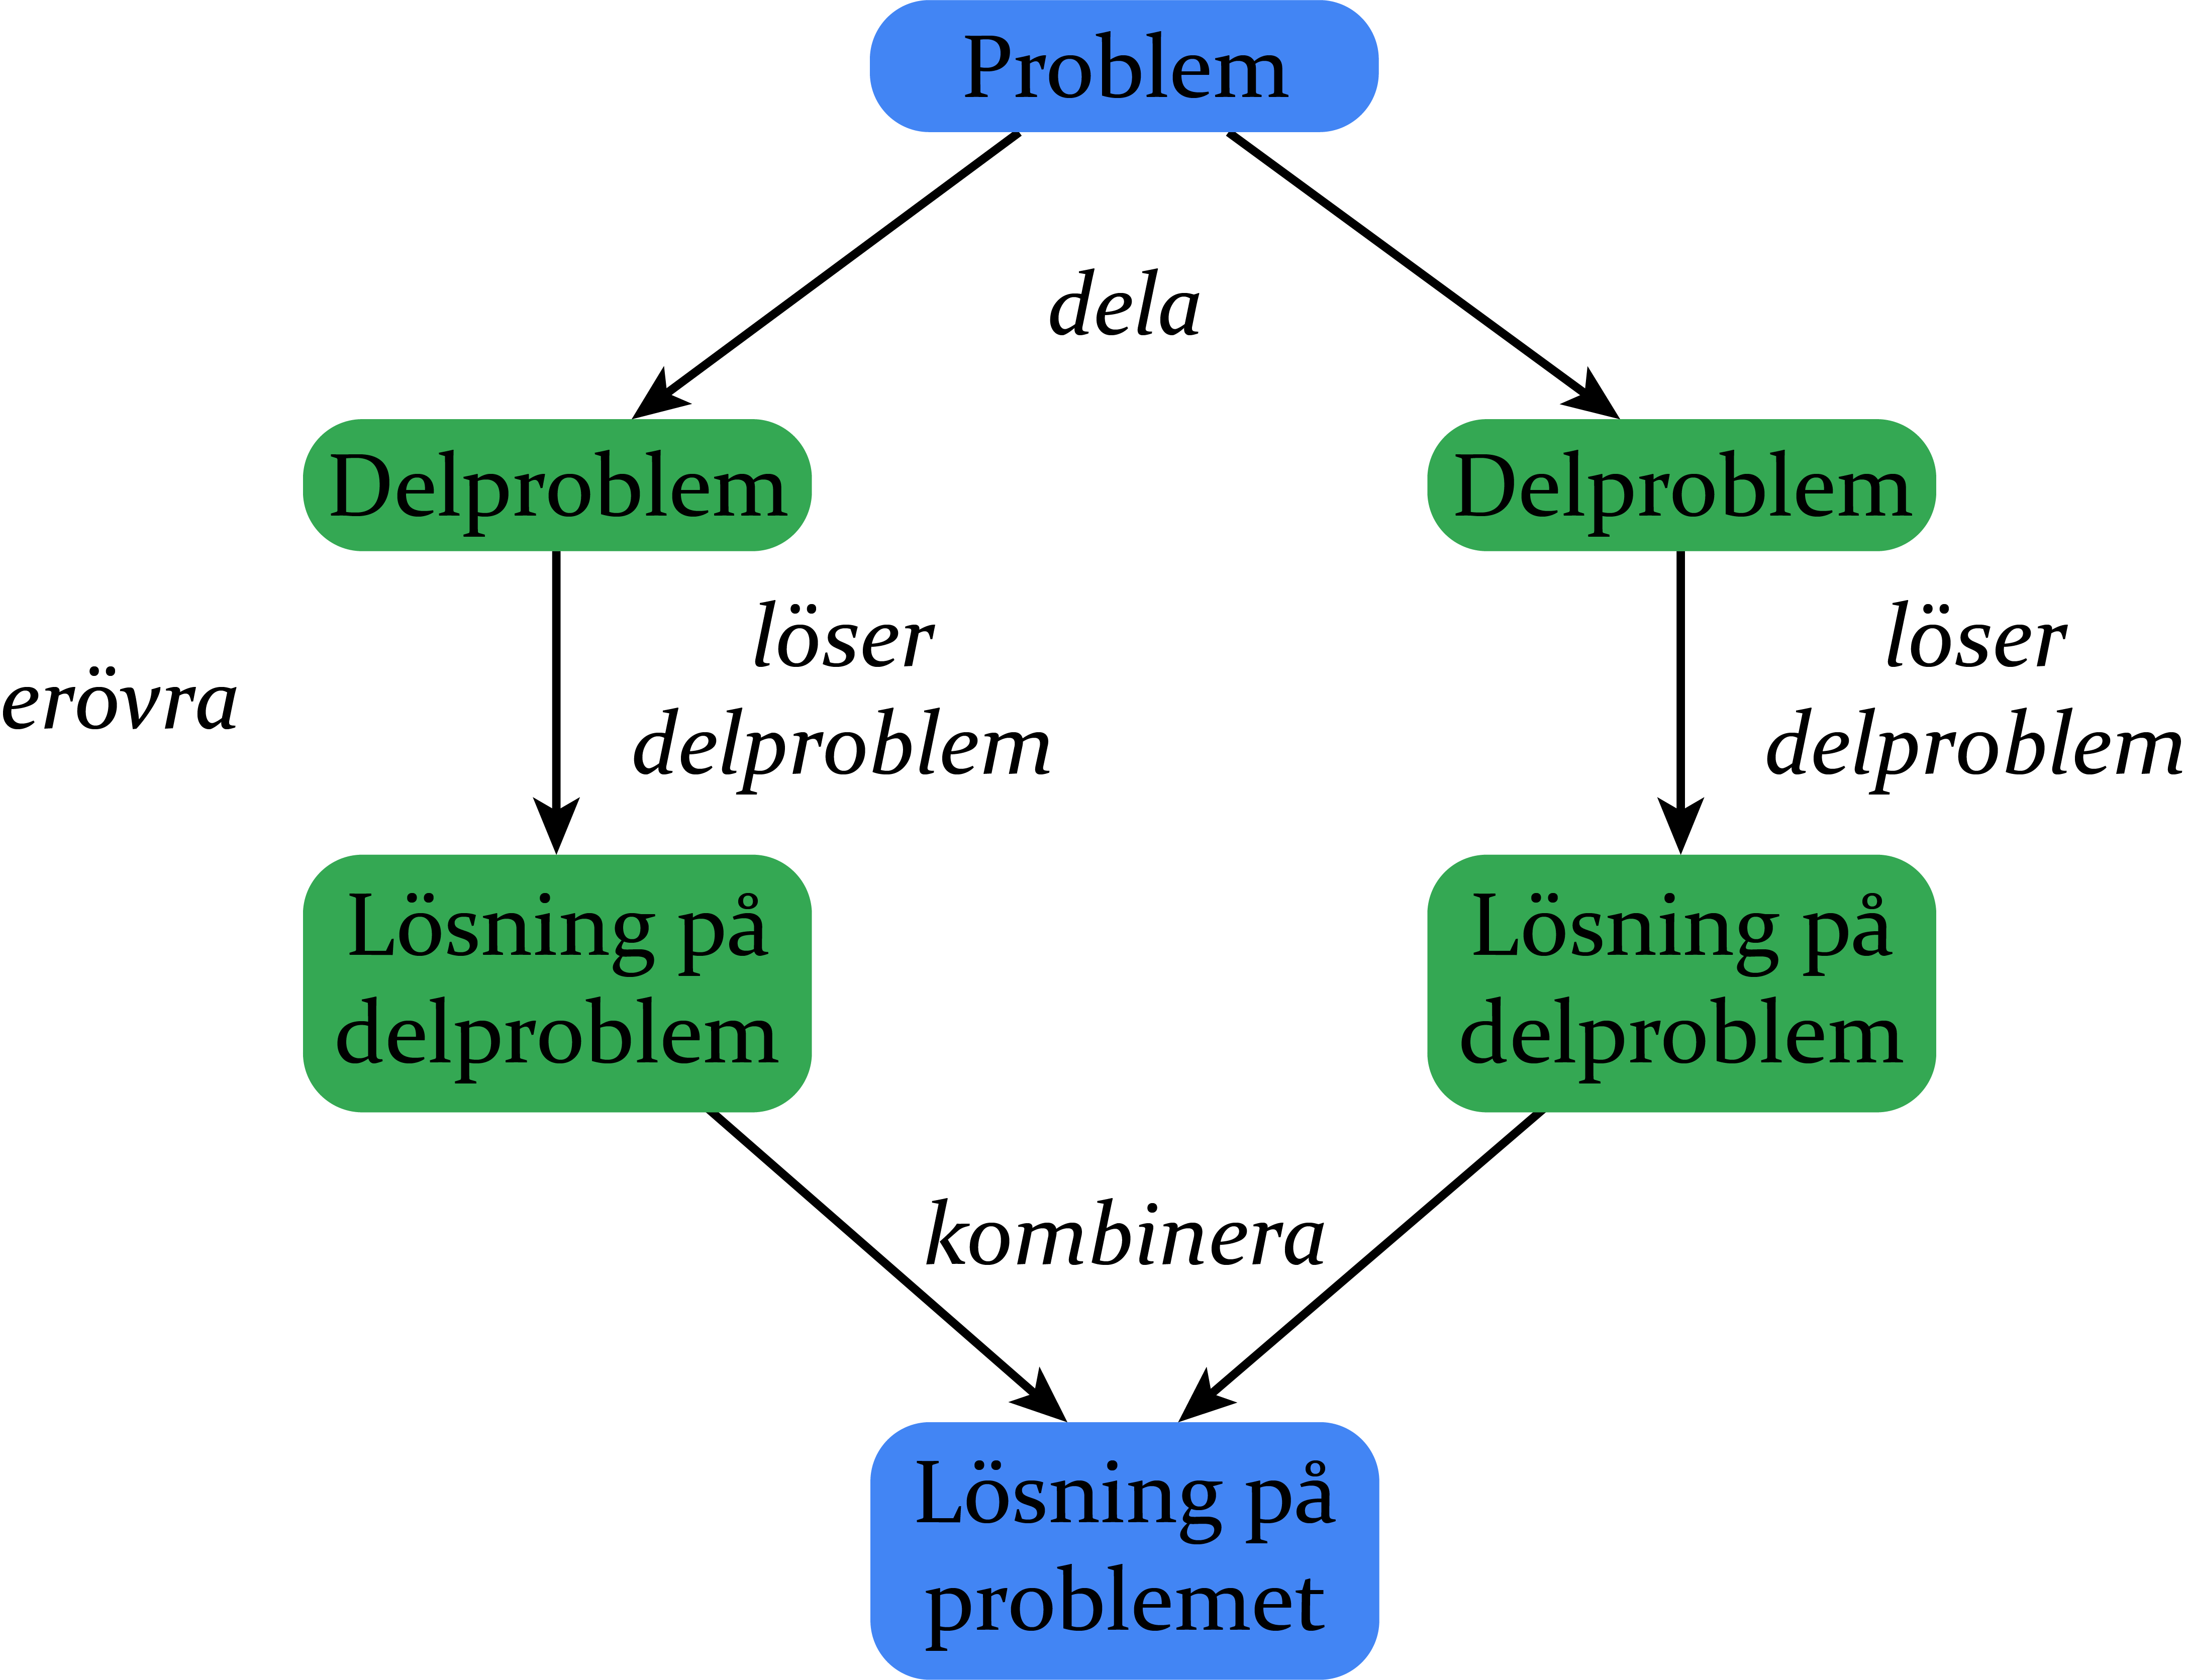
\includegraphics[scale=.15]{../../Images/DAC/DAC Diagram Small PNG.png}
\end{center}
Observera att detta är i fallet då DAC algoritmen skappar två delproblem utav det föregående problemet. Om DAC algoritm skulle lösa ett problem med två rekursioner istället för en skulle det se ut såhär: \cite{13}
\begin{center}
  \includegraphics[scale=.148]{../../Images/DAC/DAC Diagram Large PNG.png}
\end{center}

Den första divide-and-conquer algoritmen vi kommer kolla på är Quicksort. Quicksort-algoritmen utvecklades 1959 av Tony Hoare medan han var gäststudent vid Moscow State University. Vid den tiden arbetade Hoare på ett maskinöversättningsprojekt för National Physical Laboratory. I en del av översättningsprocessen behövde han sortera orden i det ryska meningarna innan han kunde kolla upp dom individuella orden i ett rysk-engelskt lexikon (lexikonet var i alfabetisk ordning på magnetisk tejp) \cite{14}. Efter han insåg att hans första idee, insertionsort, skulle vara för långsam för att sortera orden kom han på ideen för quicksort \cite{15}. Quicksort fungerar genom att först dela en given array i två mindre sub-arrayer: det mindre elementen och det större elementen. Efter det sorterar den sub-arrayerna rekursivt. Stegen för sorteringen är det följande:
\begin{enumerate}
    \item Välj ett element, kalla den för \textit{the pivot}, från arrayen.
    \item Partitionering: ändra ordningen på arrayen sådan att element med mindre värden än the pivot kommer innan the pivot och vice versa för det större elementen (element med samma värde som the pivot kan gå till båda sidor). Efter partitioneringen är the pivot på dess slutliga position. 
    \item Tillämpa stegen ovan rekursivt på sub-arrayerna med element med mindre värden och på sub-arrayerna med element med större värden.
\end{enumerate}
Basfallet för reduktionen är en array av storlek noll eller ett då det är sorterade per definition, så det kräver ingen sortering. Hur man väljer the pivot och hur man partitionerar arrayen kan göras på ett flertal sätt; vilket har stor påverkan algoritmens hastighet. Låt oss säga att vi har en array
\begin{lstlisting}[style=mystyle, numbers=none]
  intp[] lista = {3, 7, 8, 5, 2, 1, 9, 5, 4};
\end{lstlisting}
som ska sorteras med quicksort. Den fulla sortering skulle se ut såhär (the pivot är skrivet i fetstil)
\begin{center}
  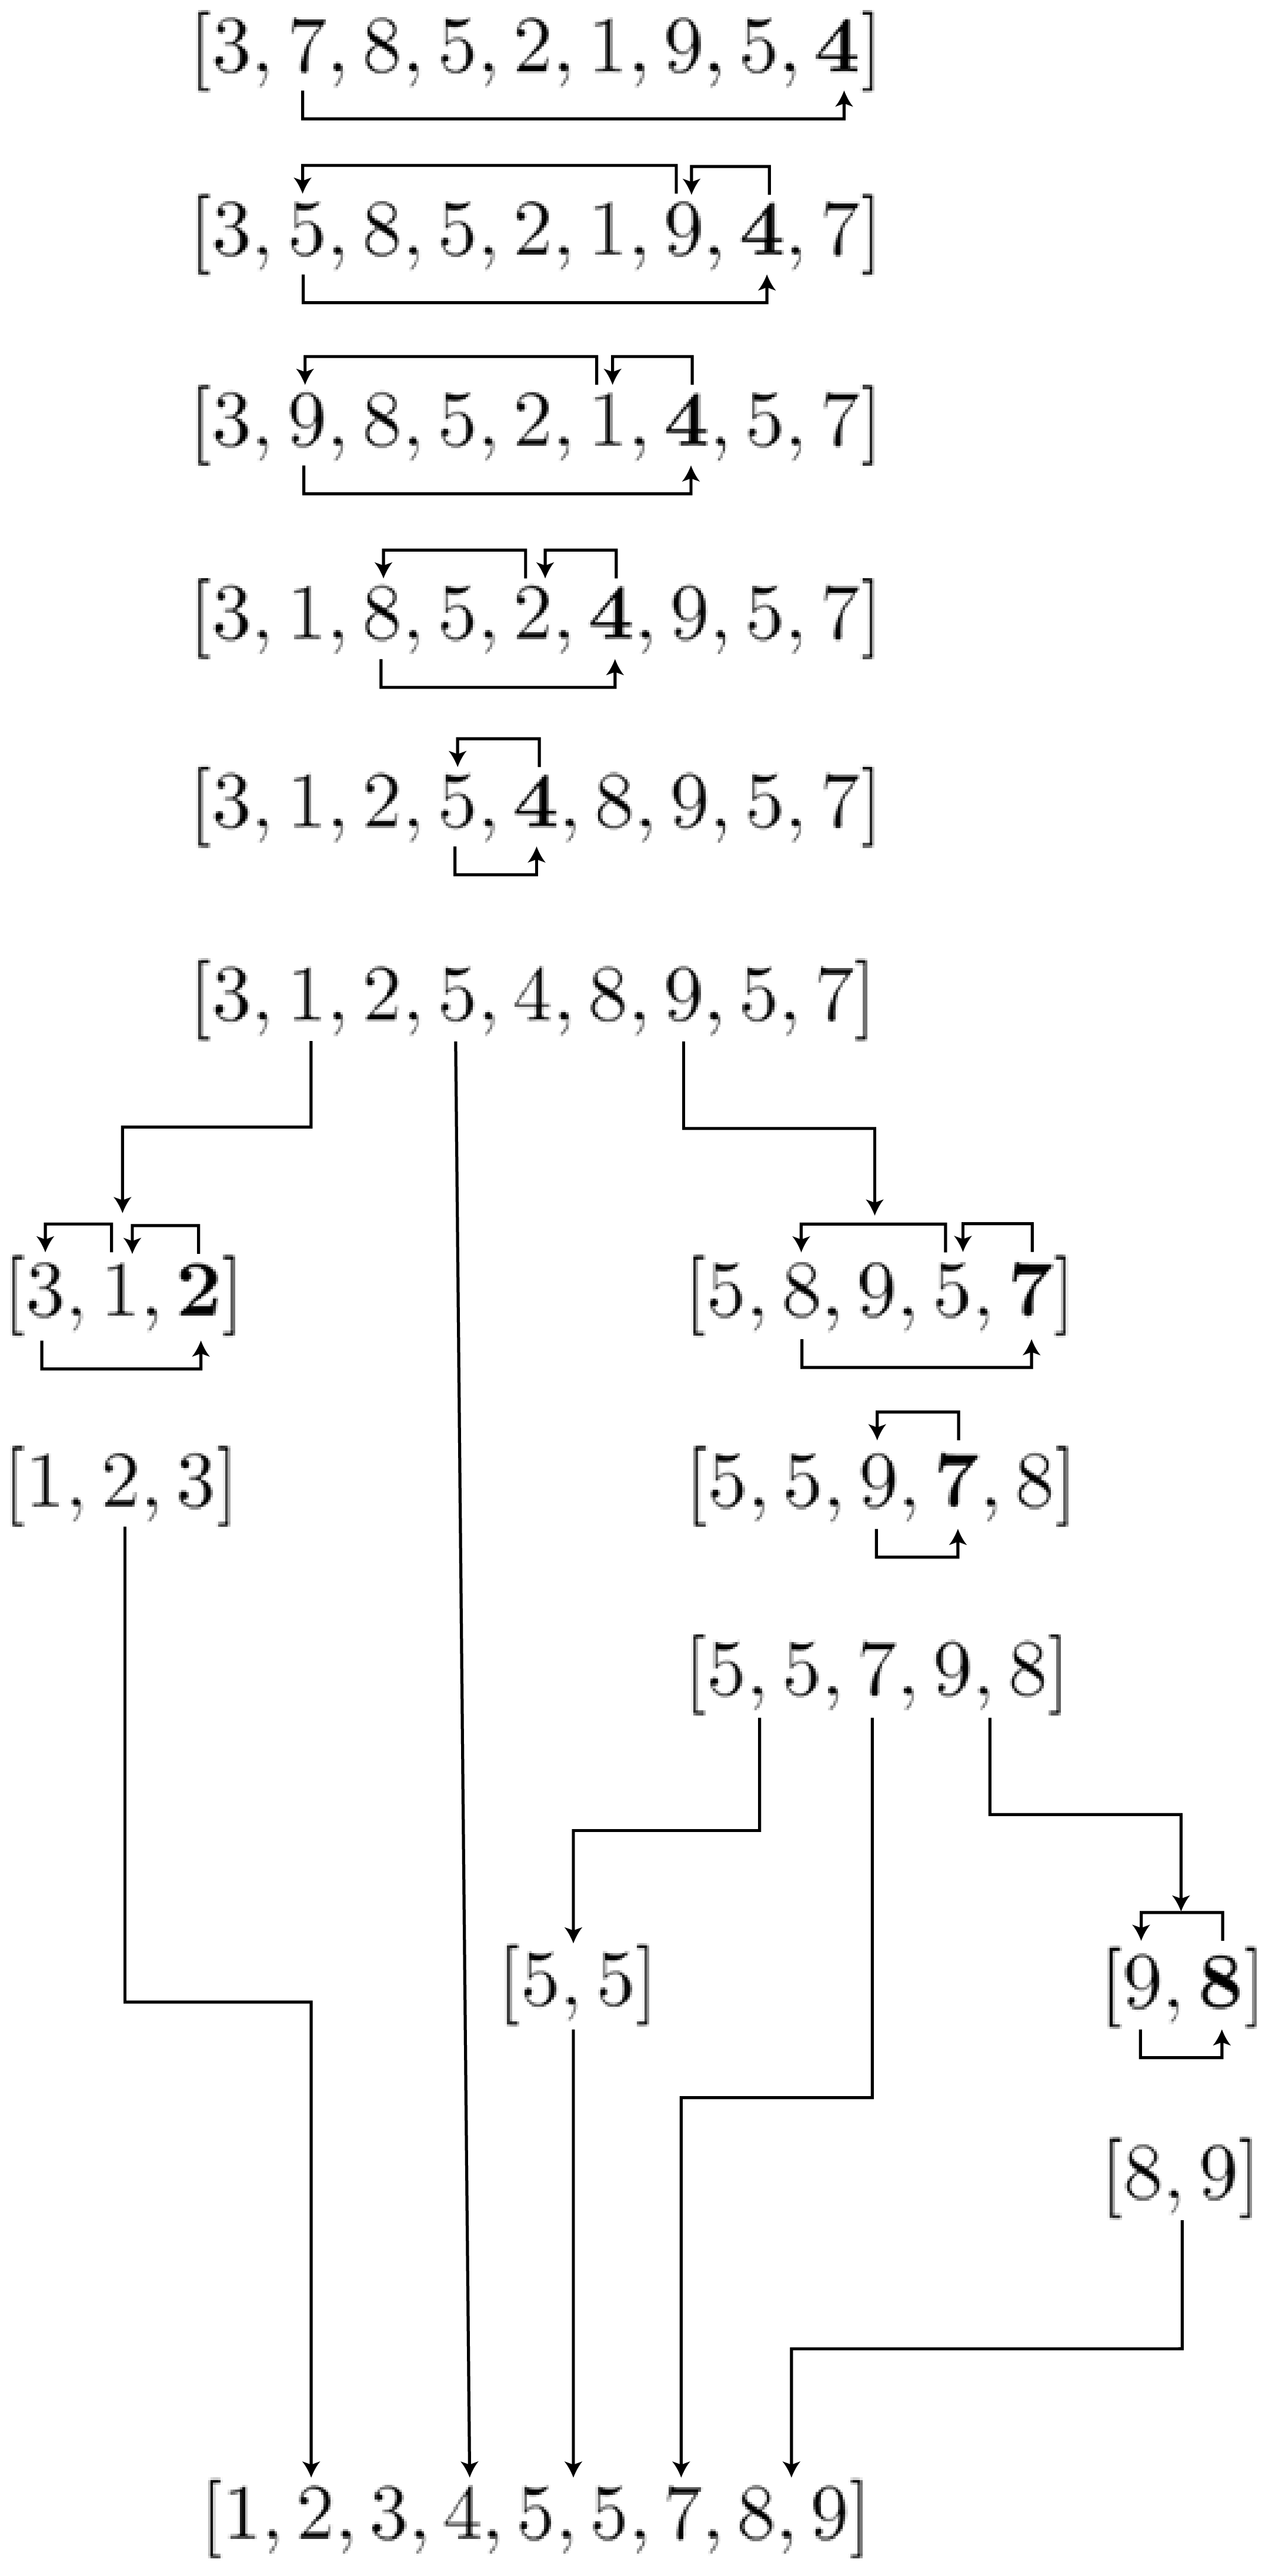
\includegraphics[scale=.29]{../../Untitled-1.png}
\end{center}



\subsection{'Jämförelse på plats' algoritmer (\#3)}

\subsection{Övriga algoritmer (\#4)}

\chapter{Metod}

\chapter{Resultat}

\chapter{Diskussion och slutsatser}

\newpage
\chapter{Källförteckning}
\printbibliography

\end{document}